\subsection{Pengujian Pengiriman Citra Kamera pada \emph{Real Robot}}
\label{subsec:citrarobot}

\begin{figure}[ht]
  \centering
  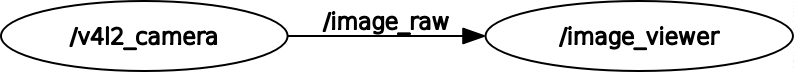
\includegraphics[width=0.95\textwidth,keepaspectratio]{gambar/rosgraph-camera.png}
  \caption{Relasi antar-\emph{node} dari pengujian pengiriman citra kamera pada \emph{real robot}.}
  \label{fig:rosgraphcamera}
\end{figure}

Sama seperti pengujian sebelumnya yang ada di bagian \ref{subsec:citrasimulasi},
  pengujian ini juga dilakukan dengan menjalankan \emph{image viewer node} dan \emph{command-line} \lstinline{$ ros2 topic}.
Hanya saja, sebagai ganti dari \emph{node} \lstinline{/camera_plugin} yang ada di simulasi,
  data citra kamera yang dikirim akan berasal dari \emph{V4L2 camera node}.
Seperti yang dapat dilihat pada gambar \ref{fig:rosgraphcamera},
  \emph{node} \lstinline{/v4l2_camera} akan mengirimkan \emph{topic} \lstinline{/image_raw} yang berisi citra kamera,
  setelah itu \emph{node} \lstinline{/image_viewer} akan menerima citra tersebut dan menampilkannya dalam bentuk GUI.

\begin{longtable}{|c|c|c|c|c|}
  \caption{Hasil \emph{delay} dan frekuensi dari pengiriman citra kamera pada \emph{real robot}.}
  \label{tb:pengirimancitrarobot}
  \\ \hline \rowcolor[HTML]{E0E0E0}
  Width & Height & Size (kb) & Delay (ms) & Rate (hz)
  \csvreader[head to column names]{data/pengiriman_citra_robot.csv}{}{
    \\ \hline
    \width & \height & \size & \delay & \rate
  }
  \\ \hline
\end{longtable}


Pengujian ini dilakukan dengan berbagai macam konfigurasi resolusi citra yang dikirim.
Hasil pengujian ini bisa dilihat pada tabel \ref{tb:pengirimancitrasimulasi}.
Sama seperti pengujian yang ada di simulasi, pada tabel tersebut \emph{width} dan \emph{height} merupakan resolusi citra yang dikirimkan,
  \emph{size} merupakan hasil perkalian resolusi dengan jumlah \emph{channel},
  \emph{delay} merupakan selang waktu yang dibutuhkan sebelum citra sampai ke penerima,
  dan \emph{rate} merupakan frekuensi pengiriman citra.


\begin{figure}[ht]
  \centering
  \begin{tikzpicture}
    \begin{axis}[
        height=0.38\textwidth,
        width=0.9\textwidth,
        ylabel=Delay (ms),
        ymajorgrids,
        ymin=0,
        ymax=40,
      ]
      \addplot table[x=size,y=delay,col sep=comma]{data/pengiriman_citra_robot.csv};
    \end{axis}
  \end{tikzpicture}
  \begin{tikzpicture}
    \begin{axis}[
        height=0.38\textwidth,
        width=0.9\textwidth,
        xlabel=Data Size (KB),
        ylabel=Rate (hz),
        ymajorgrids,
        ymin=0,
        ymax=40,
      ]
      \addplot table[x=size,y=rate,col sep=comma]{data/pengiriman_citra_robot.csv};
    \end{axis}
  \end{tikzpicture}
  \caption{Grafik \emph{delay} dan frekuensi dari pengiriman citra pada \emph{real robot}.}
  \label{fig:grafikpengirimancitrarobot}
\end{figure}


Dari data yang dihasilkan oleh pengujian ini dapat diketahui bahwa data yang dikirimkan memiliki \emph{delay} sebesar 0-14 ms serta frekuensi sebesar 5.0-30.0 hz.
Lebih lanjut, ketika hasil yang didapatkan ditampilkan sebagai grafik seperti yang terlihat pada gambar \ref{fig:grafikpengirimancitrarobot},
  seperti kesimpulan pada pengujian sebelumnya,
  hasil yang didapatkan menunjukkan bahwa semakin besar ukuran data yang dikirimkan,
  maka \emph{delay} yang dihasilkan akan cenderung naik dan frekuensi yang dihasilkan akan cenderung turun.
Walaupun cenderung naik, pada pengiriman dengan data ukuran terbesar,
  nilai \emph{delay} yang dihasilkan tersebut terhitung rendah, hanya sebesar 14 ms.
Sedangkan untuk frekuensi,
  hingga batas resolusi 640 x 480,
  pengiriman citra yang dilakukan bisa menghasilkan frekuensi diatas 90\% dari nilai FPS yang dimiliki kamera pada \emph{real robot}.
